% =====================================================================
%  Mục 7 thay thế cho bài chung (Lam, Khiem, Tan, Phuc, Phat, Ngan).
%  Dán đè toàn bộ Section 7 hiện tại ("Controlled New-Item Experiment").
%
%  Ký hiệu dùng đúng theo bài chung: a_u, b_i (Eq. 8), k_u, k_i, k_c, Eq. (14).
%  Khoá trích dẫn: đổi cho khớp .bib của bài chung — ở đây dùng
%    harper2015 (MovieLens [10]), koren2008 ([13]), krichene2020 ([15]),
%    melville2002 ([18]), do2020 ([7]), tarek2022 ([25]), ohwsf2025 ([20]),
%    slarec2026 ([3]), mrazova2023 ([19]).
%  Hình: fig_newitem_ablation.pdf, sinh bởi fig_newitem_ablation.py.
%  Mọi con số là trung bình 10 seed của hai lần chạy ablation_ml / ablation_ta
%  (16–17/11/2026); không dùng số của lần chạy cũ.
% =====================================================================
\section{Controlled New-Item Experiment}
\label{sec:newitem}

On Tripadvisor under the temporal split, very few new hotels appear in the test year and the selected value is $k_i = 0$, so the item-wise factor $b_i$ of Eq.~(8) is not put to the test there. This section therefore creates new items in a controlled way, on two datasets, and isolates what each part of the two-sided rule contributes. The protocol differs from the previous sections: the task is to predict star ratings, the hybrid has three components (collaborative, content and demographic), and cold start is induced by holding out items and truncating user histories.

\subsection{Setup}

\paragraph{Datasets.} The first dataset is MovieLens~100K~\cite{harper2015}: 943 users, 1{,}682 items and 100{,}000 ratings, with genres as content features and age, gender and occupation as demographic attributes. The second is the Tripadvisor corpus of Section~3, restricted to reviews with an overall rating and to users with at least five reviews, which leaves 382{,}279 ratings by 50{,}009 users on 3{,}131 hotels. Content features are TF-IDF vectors over star class, amenities, languages, size band and region; the demographic component uses the reviewer's home region and most frequent trip type, since the corpus carries no age, gender or occupation.

\paragraph{Components and rule.} Three component models produce a score on the rating scale: SVD++~\cite{koren2008} with 50 latent factors, a TF-IDF content model whose user profile is the rating-weighted mean of the consumed items, and a demographic model that returns the mean rating of the user's demographic group for the item, shrunk towards the item mean with a pseudo-count of~5. They are combined as $\hat{s}_{u,i} = \alpha\, s^{\mathrm{CF}} + \beta\, s^{\mathrm{CB}} + \gamma\, s^{\mathrm{DM}}$ with
\begin{equation}
  \alpha = a_u b_i, \qquad
  \beta = (1-\alpha)\,\pi_u, \qquad
  \gamma = (1-\alpha)\,(1-\pi_u), \qquad
  \pi_u = \frac{n_u}{n_u + k_c},
  \label{eq:newitem-rule}
\end{equation}
which uses the same collaborative weight $a_u b_i$ as Eq.~(8), with the demographic model as the unconditional fallback. When $m_i = 0$ we set $\gamma = 0$ and $\beta = 1 - \alpha = 1$: an item nobody has rated receives the same prior-dominated demographic value as every other such item, so blending it in cannot separate new items from one another and only dilutes the content signal that can.

\paragraph{Cold-start simulation.} Per seed, 20\% of items are drawn at random and \emph{all} of their ratings are moved to the held-out split, so these items have $m_i = 0$ in training; 30\% of users are drawn at random and only their first $n$ ratings in chronological order are kept, with $n$ uniform in $\{0,\dots,19\}$; the remaining users contribute 20\% of their ratings to the held-out split, which is then halved into validation and test. Every result is the mean over ten seeds.

\paragraph{Tuning and metrics.} All compared methods are tuned by the same grid search on the validation split, selecting by RMSE. For the rule the grid is $k_u \in \{5,10,20,40,80,160\}$, $k_i \in \{5,20,50,100,200,400\}$, $k_c \in \{1,3,10,30\}$; the modal selection is $(80,5,10)$ on MovieLens and $(40,5,1)$ on Tripadvisor, and the upper end of the $k_i$ grid is never chosen. Ranking metrics use the full catalogue of items the user has not rated~\cite{krichene2020}; on Tripadvisor they are computed on 2{,}000 sampled test users per seed. New@10 is the fraction of top-10 slots occupied by items with $m_i = 0$. Baselines are four single-paradigm models, three fixed-weight hybrids ($\alpha \in \{0.3, 0.5, 0.7\}$, remainder split 70/30) and four published hybrids~\cite{tarek2022,do2020,ohwsf2025,slarec2026}, reimplemented inside the same harness; their published numbers come from other datasets and splits and are not comparable. Differences are tested with a two-sided Wilcoxon signed-rank test over the ten per-seed values.

\subsection{Results}

\begin{table}[t]
  \caption{Controlled new-item experiment, mean over ten seeds. New@10 is the fraction of top-10 slots filled by items with no training ratings. Best value per column in bold.}
  \label{tab:newitem}
  \centering
  \small
  \setlength{\tabcolsep}{4.5pt}
  \begin{tabular}{l ccc ccc}
    \toprule
    & \multicolumn{3}{c}{MovieLens 100K} & \multicolumn{3}{c}{Tripadvisor} \\
    \cmidrule(lr){2-4}\cmidrule(lr){5-7}
    Method & RMSE & NDCG@10 & New@10 & RMSE & NDCG@10 & New@10 \\
    \midrule
    Popularity                 & 1.0806 & 0.0360 & 0.0000 & 0.9459 & 0.0026 & 0.0000 \\
    Demographic-only           & 1.0829 & 0.0401 & 0.0000 & 0.9477 & 0.0031 & 0.0000 \\
    Content-only               & 1.0215 & 0.0398 & 0.0016 & 0.9175 & 0.0030 & 0.0008 \\
    CF-only (SVD++)            & 1.0306 & 0.0447 & 0.0000 & 0.9200 & \textbf{0.0033} & 0.0000 \\
    Fixed $\alpha = 0.3$       & 1.0161 & 0.0443 & 0.0000 & \textbf{0.9104} & 0.0029 & 0.0000 \\
    Fixed $\alpha = 0.5$       & 1.0169 & 0.0455 & 0.0000 & 0.9117 & 0.0029 & 0.0000 \\
    Fixed $\alpha = 0.7$       & 1.0204 & 0.0457 & 0.0000 & 0.9141 & 0.0029 & 0.0000 \\
    Tarek et al.~\cite{tarek2022} & 1.0206 & 0.0424 & 0.0000 & 0.9135 & 0.0028 & 0.0000 \\
    Do et al.~\cite{do2020}    & 1.0192 & 0.0432 & 0.0000 & 0.9125 & 0.0029 & 0.0000 \\
    OHWSF~\cite{ohwsf2025}     & 1.0305 & 0.0443 & 0.0000 & 0.9163 & 0.0030 & 0.0000 \\
    SL-ARec~\cite{slarec2026}  & 1.0155 & \textbf{0.0504} & 0.0031 & 0.9109 & 0.0030 & 0.0001 \\
    \midrule
    Two-sided rule, Eq.~\eqref{eq:newitem-rule} & \textbf{1.0148} & 0.0480 & \textbf{0.0118} & 0.9151 & 0.0029 & \textbf{0.0024} \\
    \bottomrule
  \end{tabular}
\end{table}

Table~\ref{tab:newitem} reports the mean over ten seeds. Three observations hold on both datasets. First, nine of the eleven baselines, every one except Content-only and SL-ARec, obtain a New@10 of exactly zero: across ten seeds they never place an item with $m_i = 0$ in a top-10 list. Second, the two-sided rule has the highest New@10 by a wide margin, $0.0118$ against $0.0031$ for SL-ARec on MovieLens and $0.0024$ against $0.0001$ on Tripadvisor, and the advantage is significant against every baseline on both datasets ($10/10$ seeds, $p = 0.002$ in every comparison). Third, ranking quality does not suffer: on MovieLens the rule is second on NDCG@10 behind SL-ARec and significantly above every other baseline ($p \le 0.002$), while on Tripadvisor all twelve methods lie between $0.0026$ and $0.0033$ and no pair differs significantly.

On rating error the two datasets disagree. On MovieLens the rule attains the lowest RMSE of the twelve methods, significantly below every baseline except SL-ARec ($6/10$ seeds, $p = 0.275$, no claim made). On Tripadvisor it does not: the fixed blend with $\alpha = 0.3$ is best at $0.9104$ and the rule ranks ninth at $0.9151$, a deficit of $0.002$ to $0.005$ against the fixed-weight and published hybrids that is significant on all ten seeds. The cause is the same one seen in Section~6.3. The errors of the collaborative and content components are correlated at $0.975$ on these data (never below $0.974$ on any seed), so changing the mixing ratio barely changes the prediction: sweeping the collaborative weight from $0$ to $0.4$ moves RMSE by $0.001$, and the nine hybrid configurations span only $0.006$. With a median of four training ratings per test user and a median item count of zero, the product rule assigns a mean collaborative weight of $0.045$, below the RMSE-optimal value of about $0.2$; the rule's caution is right for ranking, where CF cannot order unseen items, and slightly costly for rating error, where SVD++ still estimates user and item biases from a handful of ratings.

\subsection{Ablation of the Two-Sided Rule}
\label{sec:newitem-ablation}

\begin{table}[t]
  \caption{Ablation of the rule, mean over ten seeds. Rows 2--3 keep the $\gamma = 0$ rule and change only how $\alpha$ is formed; row 4 keeps the product and removes that rule. Each variant is re-tuned by the same grid search.}
  \label{tab:newitem-ablation}
  \centering
  \small
  \setlength{\tabcolsep}{4.5pt}
  \begin{tabular}{l ccc ccc}
    \toprule
    & \multicolumn{3}{c}{MovieLens 100K} & \multicolumn{3}{c}{Tripadvisor} \\
    \cmidrule(lr){2-4}\cmidrule(lr){5-7}
    Variant & RMSE & NDCG@10 & New@10 & RMSE & NDCG@10 & New@10 \\
    \midrule
    $\alpha = a_u b_i$ (the rule)                 & 1.0148 & 0.0480 & \textbf{0.0118} & 0.9151 & 0.0029 & \textbf{0.0024} \\
    $\alpha = a_u$ (user side only)               & 1.0173 & 0.0456 & 0.0074 & \textbf{0.9132} & 0.0028 & 0.0000 \\
    $\alpha = (a_u + b_i)/2$                      & 1.0150 & 0.0474 & 0.0075 & 0.9142 & 0.0028 & 0.0000 \\
    $\alpha = a_u b_i$, without the $\gamma = 0$ rule & \textbf{1.0114} & 0.0476 & 0.0011 & 0.9116 & 0.0029 & 0.0001 \\
    \bottomrule
  \end{tabular}
\end{table}

\begin{figure}[t]
  \centering
  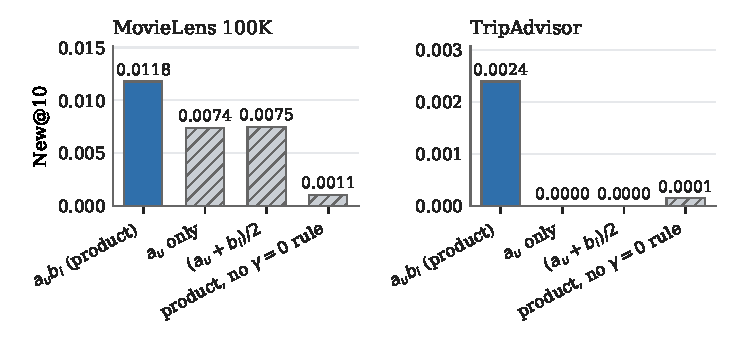
\includegraphics[width=0.95\linewidth]{fig_newitem_ablation}
  \caption{New@10 of the four variants of Table~\ref{tab:newitem-ablation}, mean over ten seeds. On Tripadvisor only the product with the $\gamma = 0$ rule places any unrated hotel in a top-10 list.}
  \label{fig:newitem-ablation}
\end{figure}

Table~\ref{tab:newitem-ablation} and Fig.~\ref{fig:newitem-ablation} isolate the two design choices. Replacing the product by the user-side factor alone, the form used by Melville et al.\ and Do et al.~\cite{melville2002,do2020} and by the schedule evaluated in the companion HotelRec study, lowers New@10 from $0.0118$ to $0.0074$ on MovieLens and from $0.0024$ to exactly $0.0000$ on Tripadvisor. The Tripadvisor outcome is the one the construction predicts: an established user has $a_u$ close to one, so a user-side rule hands the full collaborative weight to a hotel the CF model has never seen, and content similarity never gets to rank it. Averaging the two factors behaves the same way, since a mean cannot drive $\alpha$ to zero when only one side is empty. Both alternatives are worse on New@10 on both datasets ($10/10$ seeds, $p = 0.002$; mean of factors on MovieLens $9/10$, $p = 0.004$) and, on MovieLens, also on RMSE and NDCG@10.

Removing the $\gamma = 0$ rule while keeping the product lowers New@10 by an order of magnitude on both datasets, from $0.0118$ to $0.0011$ and from $0.0024$ to $0.0001$ ($10/10$ seeds, $p = 0.002$), and improves RMSE slightly ($1.0114$ and $0.9116$). The demographic component carries a little rating-scale accuracy on new items but returns a near-constant value across them, so blending it in pushes all of them below the top-10 cut-off. The two choices are therefore complementary: the product keeps an unrated item away from the collaborative model, and the $\gamma = 0$ rule hands it to the one component that can distinguish it from other unrated items. Either alone is insufficient, and on Tripadvisor the user-side and mean variants give exactly the result of Section~6, where $b_i$ is not used: no new hotel is ever recommended.

Two caveats apply. The absolute New@10 rates are small, because 20\% of the catalogue is unrated and the metric counts top-10 slots; the claim is comparative, against a floor of exactly zero. And the experiment verifies only that NDCG@10 does not fall when new items are surfaced, not that the surfaced items are the ones the user would have preferred among new items, which the data cannot tell us.
